% -----------------------------------------------
% Vlastní text práce (kapitoly práce)
% -----------------------------------------------

% -----------------------------------------------
\chapter{Astroparticle detection}
% -----------------------------------------------
More than 100 years have passed since Victor Franz Hess first encontered cosmic radiation. Since those times the techniques and methods of detection have been strongly improved. We have moved up from elevating electroscopes by ballons to observe growing electric charge to specialized techniques, which allows us to measure particles' energies, trajectories, etc.

% -----------------------------------------------
\section{Cosmic rays and particles}
% -----------------------------------------------
Cosmic rays is a term for radiation and energetic particles striking earth atmosphere with an origin in a outer space sources (neutron stars, supernovas, black holes, etc). There are two types of cosmic rays - primary and secondary. Primary cosmic rays are the original cosmic particles, which strike the Earth's athmosphere. Secondary cosmic rays (also refered as showers) are particles, which have origin in particle interaction between primary cosmic rays and the athmosphere.
\par
\begin{figure}[H]
 \centering
 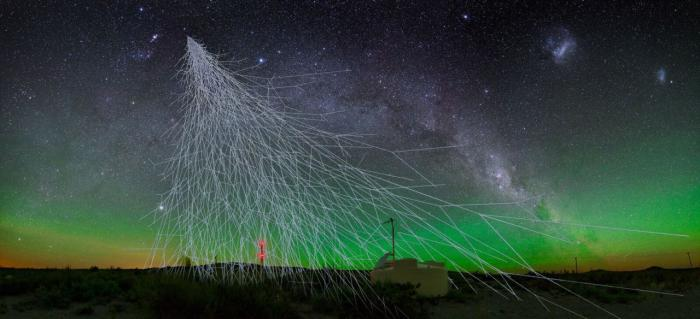
\includegraphics[scale = 0.6]{./pictures/rays}
 \caption{Ilustration of cosmic rays striking Earth's athmosphere (credit: A. Chantelauze, S. Staffi, L. Bret) \cite{intro}.}
 \label{cascade}
 
\end{figure}

\subsection{Primary cosmic rays}
Primary cosmic rays consist of protons ($95 \%$), helium nuclei ($4 \%$), electrons and other heavy nuclei (up to iron). However, only the highly energetic rays make their way to the athmosphere. The Earth's magnetic field affects their trajectories and prevents the low-energetic (less than 100 MeV) particles from arriving to the athmosphere \cite{Kliewer}. 
\par
Part of primary cosmic rays are also Ultra-high energy cosmic rays (UHECRs), which we refer in the next chapter.
\par 
Neutrinos are also a part of cosmic radiation, but their interaction with matter is very rare, so they are very hard to detect. The special underwater detectors are developed to detect some of them. 
\subsection{Secondary cosmic rays}
Secondary cosmic rays are created by interaction of high-energetic particles of primary component with air nuclei, such as nitrogen. They consist of low-energetic and high-energetic muons, gamma photons, electrons and positrons. Most of muons travel up to the earth's surface although their half-life is only about 2.2 microseconds before they decay into electrons and neutrinos. Due to their high relativistic speeds, their half-life is increased for external observers. 




% -----------------------------------------------
\section{Ultra-high energy cosmic rays (UHECRs)}
UHECRs are particles with energies from $10^{18}$ to $10^{20}$ eV, which is much more than particles created on Cern's Large hadron colider (LHC) with energies about $10^{13}$. Due to their high energies, the trajectory remains nearly unchanged by space magnetic fields \cite{Benjamin_Skuse}.
\par
UHECRs' origin is yet unknown, but it is supposed and experimentally proved that they come from outside of the Milky Way. Some theoretical physicists expect, that the one possible source of UHECRs acceleration are the starburst galaxies. One of UHECR possible particle is proton. 
\par
In many particle physics experiments, some form of calorimeter is used to determine the particles' energy and direction. In case of UHECRs, the air molecules of athmosphere have the function of calorimeter.
When UHECR interacts with athmospheric nuclei, the cascade of particles is induced. This cascade concists of three main components: electromagnetic, hadronic and muonic. It is also refered to as extensive air shower (EAS).
\par
In case of ultra-high energy proton striking an air molecule, kaons, baryons, nuclear fragments and mostly pions are created. Together, they are refered as hadronic component. The pions with short lifetime decay into electromagnetic sub-shower. The behaviour of pions with longer lifetime is energy-dependent. At higher energies they reinteract with atmospheric nuclei and feed hadronic and electromagnetic component. At lower energies they decay into muonic component with muonic neutrinos. The muons with short lifetime decay into electrons and positrons with neutrinos, which join the electromagnetic cascade, while the others reach the Earth's surface carrying the energy, which we are unable to detect (invisible energy). The UHECR's cascade scheme is shown in Fig. \ref{cascade}. 
\begin{figure}[H]
 \centering
 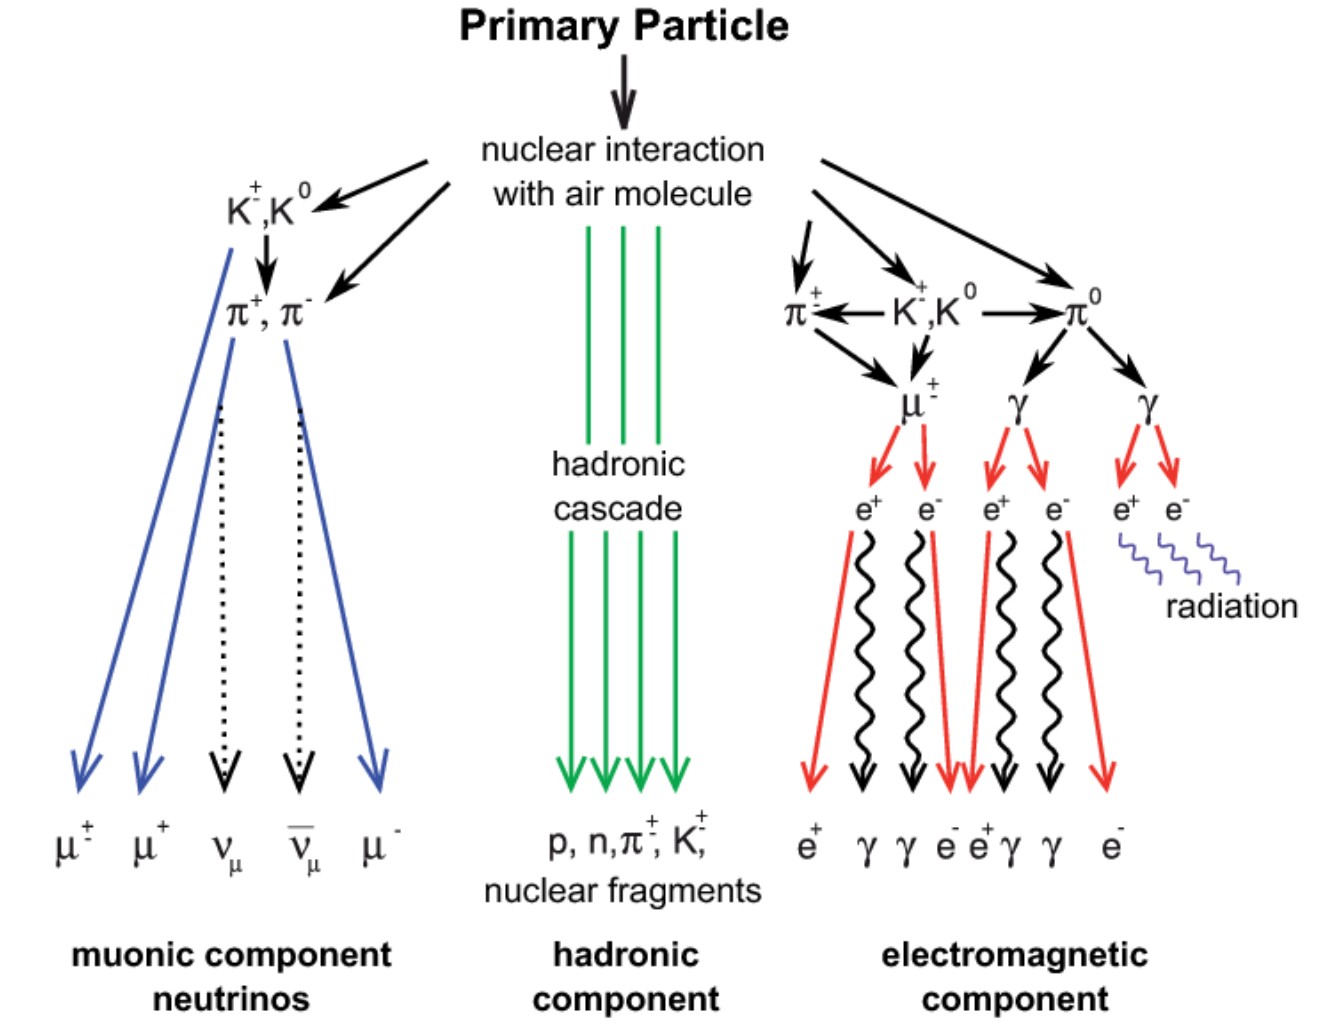
\includegraphics[scale = 0.3]{./pictures/cascade}
 \caption{UHECR's cascade, taken from \cite{Cascades}.}
 \label{cascade}
 
\end{figure}

\par

The electromagnetic cascade consisting of electron, positrons, gama photons carries the most of UHECR's energy. With increasing depth, the cascade develops by decaying the photons into electron and positron pairs, which again emit photons and this process repeats. The cascade develops until the the energy treshold is reached, where the ionization is higher than the radiation losses. \cite{Tomankova2016_1000061954}.


\par
Every UHECR shower has its own longtitudal profile. One of the main parameters of this profile is $X_{max}$ - the point along the shower axis, where is the maximum of deposited energy. Other property which we are able to capture is the lateral distribution of particles, which has a decreasing trend with the increasing distance from the shower core. By analyzing the signal waveforms from our detectors we are also able to determine the time structure of the event.

% -----------------------------------------------
\section{UHECRs detection techniques}
Nowadays there are three main proven techniques to detect UHERCs - 
air fluorescence, surface particle detection and Cherenkov light detection. The detectors consists of the optical part (mirrors, reflectors and optical filters), the detection part (PMTs and PMT based cameras) and the electronic part. The electronic part mainly consists of special triggering and sampling systems and a data acquisition system (DAQ) capable of storing huge amounts of complex data (full signal waveforms etc.).

\subsection{Air fluorescence}
The electrons and positrons from electromagnetic cascade excite nitrogen molecules, which then deexcite and emit fluorescence light in UV spectre with two main wavelengths 337 and 357 nm. The intensity of this light is directly proportional to the calorimetric energy of the shower.
\par
However, the intensity of this light is very low, and thus the measurements must be done in dark nights with no light smog. Even a low intensity of external sources can led to detection of false events or worse - the unwanted light may damage the very sensitive equipment. 
\par
The detection equipment consists mostly the superreflective UV mirrors which focus part of the UV shower into the PMT or into the camera based on PMTs. It it necessary to have atmospheric monitoring system (temperature, humidity, pressure etc.) along with the detection part, because the fluorescence is highly dependent on these conditions.  
\par
The main advantage of fluorescence detection is the fact, that by measuring and integrating the light profile we are able to calculate the total calorimetric energy. However, corrections must be made due to the invisible energy.

\par
The FAST telescope, on which we focus in this thesis, is a fluorescence telescope.
\subsection{Surface particle detection}
Surface particle detection is a method, which is based on detecting individual particles from EAS. There are two proven surface techniques to detect EAS - by scintillators or water Cherenkov detectors. To detect the EAS full geometric distribution, huge surface needs to be covered by surface detectors. By combining the information from the multiple surface detectors we are able to obtain the footprint, direction and the total energy of the air shower.
\par
In case of Chernenkov surface detectors, the special plastic tanks filled with purified water are used. The water is used as a Chernenkov radiator, which emits the Chernenkov photons whenever the relativistic charged particle strikes the detector. This light is sampled by PMTs overseeing the water.
To increase the collection efficency, the tank's inner surface is covered by reflective material. The detector is also sensitive to the non-Chernenkov high energetic photons, which has the origin in the electron and positron anihilation in the UHECR's cascade.
\par
The second possibility is to use the detectors equipped with scintillators. Scintillator detectors are flat devices with a scintillator array in a metal clad. The scintillator consists of special molecules which are sensitive to charged particles, which are excited when striked by a charged particle. Upon deexcitation they emit UV light which is transfered to PMTs by optical fibers.
\par
Compared to fluorescence detection method, the surface detectors don't require the dark night and any light exposure is not a threat for them. Thus they are capable of operating during the entire day. 

\par
The main disadvantage of surface detection is the calibration. For solo surface detector, there is only one possibility - by using simulation models, which are mostly corrupted by many uncertanities. Better approach to solve this problem is to use the hybrid detection technique.


\subsection{Cherenkov light detection}


\subsection{Hybrid detection}
Nowadays the hybrid detection seems to be the most proven way to detect UHECRs. Both of the main UHECRs observatories - the Pierre Auger observatory and the Telescope array project both are based on the hybrid detection. 
\par
The hybrid detection allows the observatory to operate 100 $\%$ of the daytime and mainly solves the surface detector calibration problems. By comparing the event captured by both fluorescence and surface detectors we are able to transfer the energy scale from the fluorescence detectors to the surface detectors and thus calibrate the surface detectors.



\section{UHECRs observatories}
The Pierre Auger observatory is the observatory located on the southern hemisphere. It uses over 1660 Chernenkov tanks as surface detectors covering more than 3000 k$\textrm{m}_2$ of the Pampa Amarilla. 27 telescopes situated on the boards of the observatory are used as fluorescence detectors \cite{Tomankova2016_1000061954}.
\par
The Telescope array project is located on the northern hemisphere in Millard County, Utah. It consists of more than 500 scintillator detectors and  three fluorescence telescope stations \cite{Array}.


% %%%%%%%%%%%%%%%%%%%%%%%% End of file %%%%%%%%%%%%%%%%%%%%%%%%
